	\begin{frame}[c]\frametitle{Search algorithm}
		\begin{columns}
			\column{4cm}
			\begin{itemize}
				\item<1-> Search algorithm
				\item<1-> exponential : $O(x^{depth})$
			\end{itemize}
			\column{6cm}
			\only{\centering{{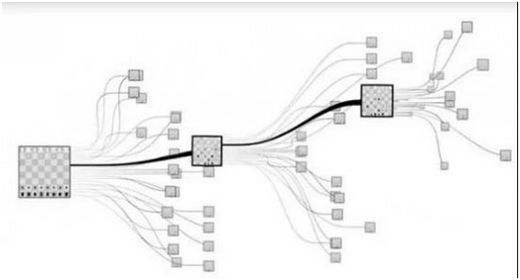
\includegraphics[width=6cm]{xzj_part/timg.jpg}<1>}}}
		\end{columns}
	\end{frame}
	\begin{frame}[c]\frametitle{Meet in the middle}
		\begin{columns}
			\column{4cm}
			\begin{itemize}
				\item<1-> Given an undirected graph whose nodes' degree is 5 and find a path from $S$ to $T$.
				\item<2-> dist(S, T) = L
				\item<3-> $O(4^L)$
				\item<4-> Meet in the middle
				\item<4-> $O(4^{L/2})$
			\end{itemize}
			\column{6cm}
			\only{\centering{{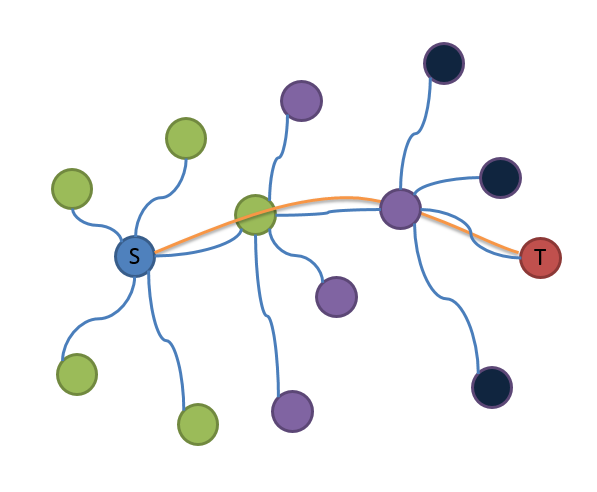
\includegraphics[width=6cm]{img/pic0.png}<1-2>}}}
			\only{\centering{{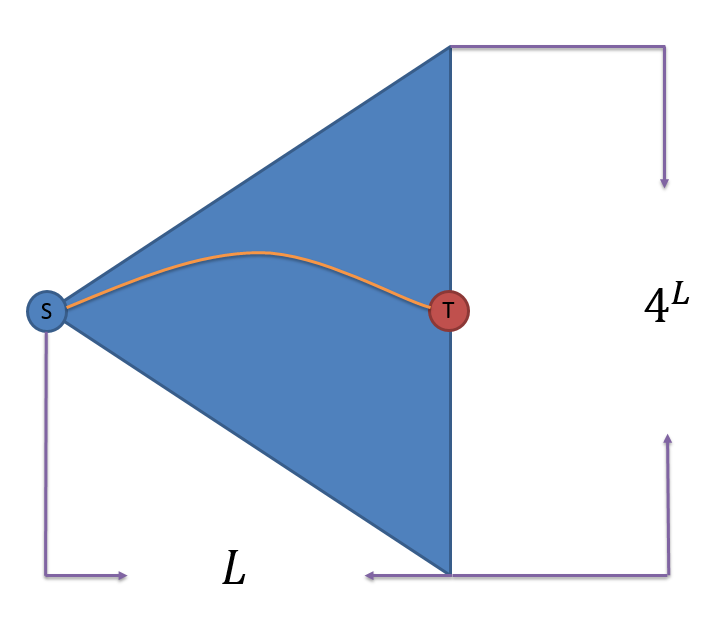
\includegraphics[width=6cm]{img/pic1.png}<3>}}}
			\only{\centering{{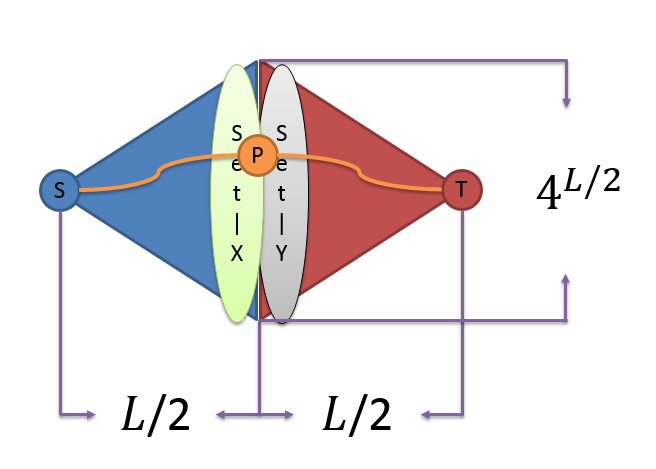
\includegraphics[width=7cm]{img/pic2.png}<4>}}}
		\end{columns}
	\end{frame}
	\begin{frame}[c]\frametitle{Some other applications}
		\begin{columns}
			\column{4cm}
			\beamerdefaultoverlayspecification{<+->}
			\begin{itemize}
				\item Mo's algorithm
				\item Blocked list
				\item Dinic(capacity is 1)
				\item ......
			\end{itemize}
			\column{7cm}
			\only{\centering{{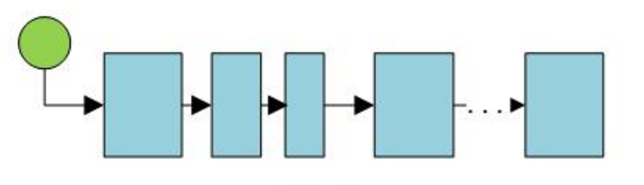
\includegraphics[width=7cm]{img/bl.png}<2>}}}
		\end{columns}
	\end{frame}
